\documentclass[a4paper]{article}

\usepackage[english]{babel}
\usepackage[utf8x]{inputenc}
\usepackage{amsmath}
\usepackage{amsfonts}
\usepackage{graphicx}
\usepackage[colorinlistoftodos]{todonotes}
\usepackage{hyperref}

\title{CS 5785 -- Applied Machine Learning -- Lec.\ 10}
\author{Prof.\ Nathan Kallus, Cornell Tech\\Scribes: TBD}
\date{Sept.\ 26, 2017 (Under construction)}

\begin{document}
\maketitle
 
\section{Naive Bayes Review}

We'll continue our discussion on Naive Bayes by working through some examples from Kevin Murphy: \url{http://www.cs.ubc.ca/~murphyk/Teaching/CS340-Fall06/lectures/naiveBayes.pdf}.  
%Kevin's notation is slightly different from what we've shown in lecture, but we'll try to make things more consistent here.
%So we'll be discussing how to use Naive Bayes for problems with continuous and discrete variables.  

\subsection{Naive Bayes with Continuous Features}
Consider the example of distinguishing cis-males and cis-females using a 2D feature vector with height and weight as shown in Figure \ref{fig:height_weight}. 
We assume Gaussian class conditional densities
$$
p(x|y=c,\theta_c) = \mathcal{N}(x|\mu_c, \Sigma_c)
$$
where the mean $\mu_c$ and covariance matrix $\Sigma_c$ depend on the class (cis-male or cis-female).
The scatter plot in Figure \ref{fig:height_weight} shows the raw data points along with covariance ellipses.

\begin{figure}
\centering
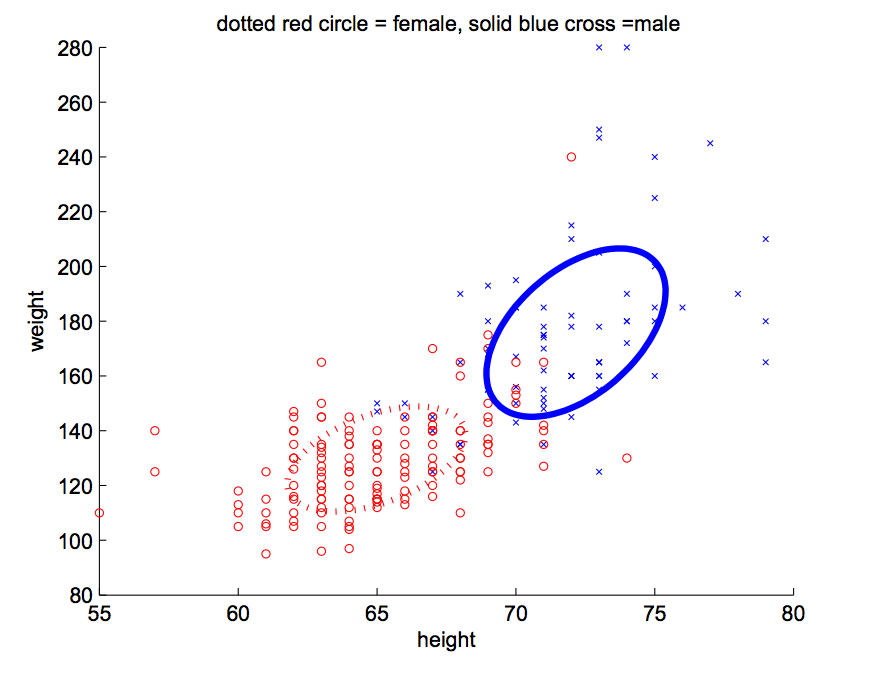
\includegraphics[width=0.75\textwidth]{fig1_murphy.png}
\caption{\label{fig:height_weight}Scatter plot of weight and height for men and women with covariance ellipses superimposed.}
\end{figure}

Although the covariance ellipses clearly show a correlation between the two variables, Naive Bayes assumes the features are independent given the class, i.e., the joint density is just a product of the individual densities:
$$
p(x|y=c,\theta_c) = \prod_{d=1}^{p} p(x_d|y=c,\theta_c) = \prod_{d=1}^{p}\mathcal{N}(x_d|\mu_{cd}, \sigma_{cd})
$$
Therefore we need only fit a univariate Gaussian to each feature variable.  
Figure \ref{fig:univariate_dist} illustrates the histograms and Gaussian fits for the individual features from each class.  Thus, the training procedure for our Naive Bayes classifier consists of estimating the mean and variance of each variable per class.


\begin{figure}
\centering
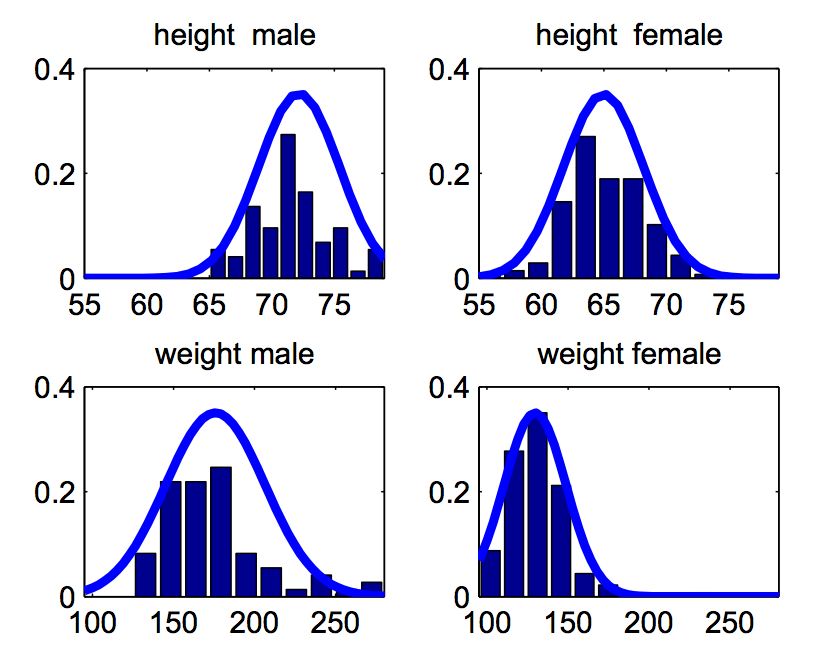
\includegraphics[width=0.75\textwidth]{fig2_murphy.png}
\caption{\label{fig:univariate_dist}Histograms and univariate Gaussian fits to each feature variable.}
\end{figure}

For testing, we apply Bayes' rule:
$$
p(y=m|x) = \frac{p(x|y=m)p(y=m)}{p(x|y=m)p(y=m) + p(x|y=f)p(y=f)}
$$
The posterior probability of the class being cis-male given the features equals the class-conditional likelihood times the prior probability over the normalization term which sums over all the possible cases.

For simplicity, we'll assume equal priors for cis-male and cis-female, i.e., $p(y=m)=p(y=f)=0.5$, which tells us that
$$
p(y=m|x) = \frac{p(x|y=m)}{p(x|y=m) + p(x|y=f)}
$$
which is, in turn, equal to
$$
p(y=m|x) = \frac{p(x_h|y=m)p(x_w|y=m)}{p(x_h|y=m)p(x_w|y=m) + p(x_h|y=f)p(x_w|y=f)}
$$
by the Naive Bayes independence assumption.
During testing you can just plug $x_h$ and $x_w$ into this expression (using the fitted normal densities for each $p(\cdot)$) and you'll get the probability of cis-male.  The probability of cis-female would be 1 minus that.

As mentioned in the previous lecture, although the Naive Bayes classifier makes unrealistic assumptions about the class conditional densities, it is surprisingly effective in practice. Also, if we would have to imagine what would a fully correct Naive Bayes would look like - it would look like a scatter plot of points which summon a perfect circle (as opposing to an oval like on Figure 1.)

\subsection{Naive Bayes with Discrete Features}
Consider the word-by-document matrix shown in Figure \ref{fig:wordbydocument}.  Each row contains a bit vector indicating presence or absence or words in a document. And $x$ represents a ``document".  If we denote a row of this matrix by the vector $x$, then $x_d=1$ means that word $d$ appears in the document at least once.  If the documents represent abstracts of scientific papers, then the classes $c$ could represent subjects (biology, chemistry, physics, etc.).

\begin{figure}
\centering
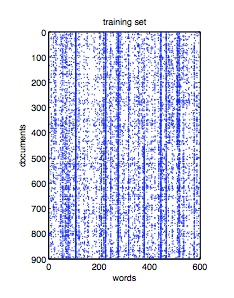
\includegraphics[width=0.5\textwidth]{fig3_murphy.png}
\caption{\label{fig:wordbydocument}Document-by-Word Matrix.  Each row is like a bag-of-words vector (i.e., histogram) thresholded to 0 or 1.}
\end{figure}

The binary outcome is a Bernoulli random variable.  Under the Naive Bayes assumption, the class-conditional densities become a product of Bernoullis with parameter $\theta_{cd}$.  So the class-conditional density -- the probability of observing a set of words in a document given that the topic is physics, for example -- is the product of the probabilities of each individual word being present in that topic.

There are a few problems, though.  If you're dealing with scientific papers, the word ``abstract" probably appears in every paper. You could argue that it's harmless but some words might throw you off (some word that has nothing to do with a scientific topic that happens to be there, like stop words). For example, if you found a movie has the word ``excellent" appeared the most in its review, they probably also came from ``the least excellent movie". You can also run into numerical underflow problems.  Murphy's slides describe in detail how to deal with this.

Recall that Naive Bayes fights the curse of dimensionality because the parameter estimation problem scales linearly with the dimensionality.  If you're modeling joint densities without an independence assumption, you have to deal with the covariances (at least) for all possible variables and the probability densities get a lot more complicated.

\section{Bag of Words}

Going back to bag of words, in Murphy's example above the vectors were binary.  If we keep the word counts we can apply Naive Bayes with Multinoulli instead of Bernoulli.  Figures \ref{fig:texture} and \ref{fig:wordcloud} show examples of bag-of-words descriptions for texture images and text, respectively.


\begin{figure}
\centering
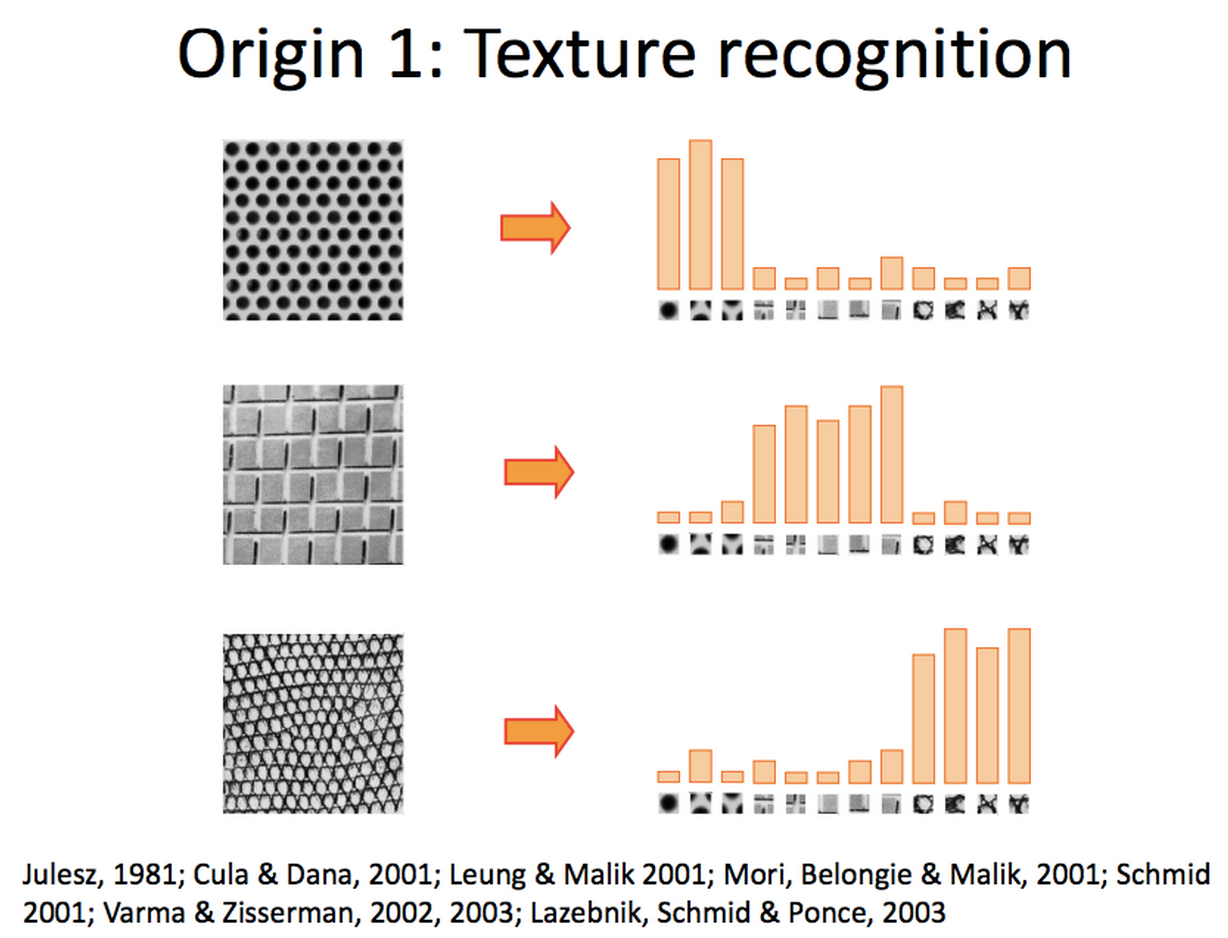
\includegraphics[width=0.8\textwidth]{fig4b_fergus.png}
\caption{\label{fig:texture}Bag-of-words descriptions of texture images using \emph{textons}.  Here, the ``words'' are vector-quantized image patches that constitute a ``vocabulary'' for images of common textures. [Fergus]}
\end{figure}

\begin{figure}
\centering
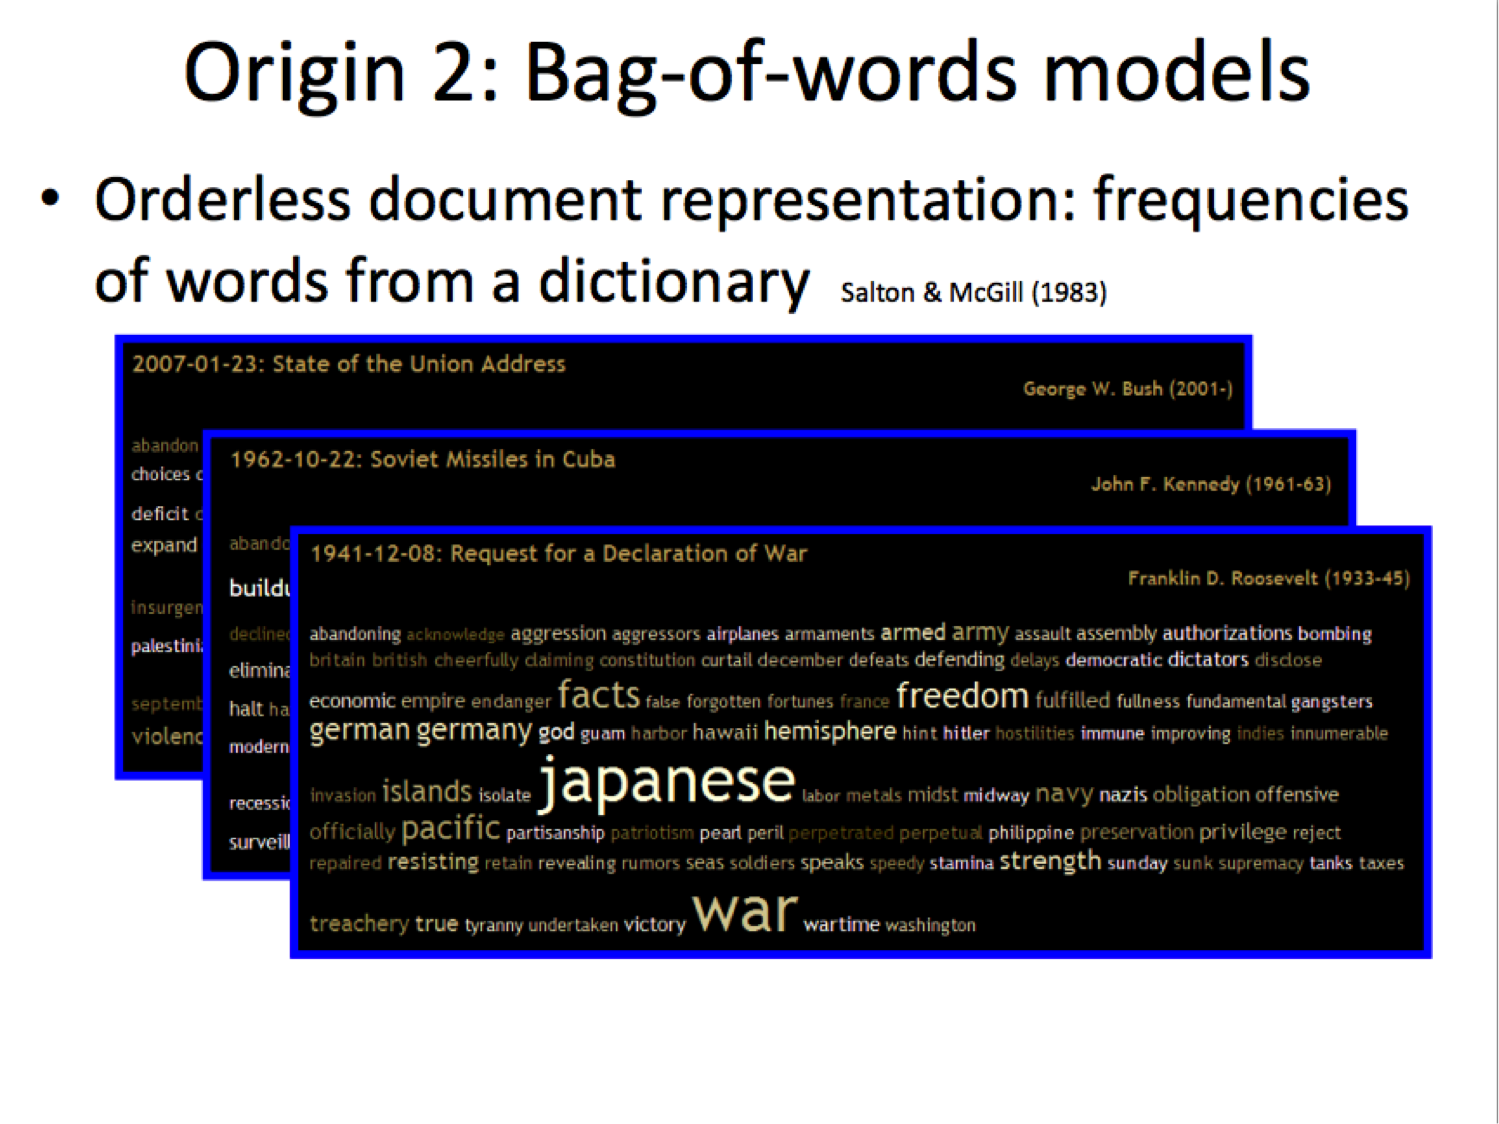
\includegraphics[width=0.8\textwidth]{fig5_fergus.png}
\caption{\label{fig:wordcloud}Word cloud visualization of bag-of-words descriptors for presidential speeches. [Fergus]}
\end{figure}

We use the term ``bag'' to convey the idea that we're not paying attention to the order of the words (texton matters, not the ordering).  Naive Bayes gives us a simple means of training classifiers and estimating per class probabilities for unknown test examples. In BoW, $E$,$F$ are normalized histogram vectors that containing word frequency. 
But what if you just want to compare two things?  How do we compare them? In the case of classification, there's a well-defined training step per class, requiring collection of labeled examples and estimating parameters to characterize each class.  With pairwise comparison, there is no training step, one needs only a measure of similarity or dissimilarity.  

\section{Pairwise Similarity}

\subsection{Chi-Squared Test}
The chi-squared test measures the dissimilarity between an empirical histogram and a reference pdf through the following expression
$$
\chi^2 = \sum_{i=1}^{K} \frac{(F_i - E_i)^2}{E_i}
$$
where $F_i$ is the empirical count in bin $i$, $E_i$ is the theoretical count in bin $i$, and $K$ is the number of bins.  We model the error as a $\chi^2$ random variable with $K-1$ degrees of freedom., i.e., the pdf of the sum of $\mathcal{N}(0,1)$-distributed random variables.  This is illustrated for the case of a Gaussian pdf in Fig.\ \ref{fig:chisq}.  The $\chi^2$ test simply adds up the squared error between the measured and theoretical bin counts, normalized by the theoretical bin count.  As such, relative differences between the counts play an important role.


\begin{figure}
\centering
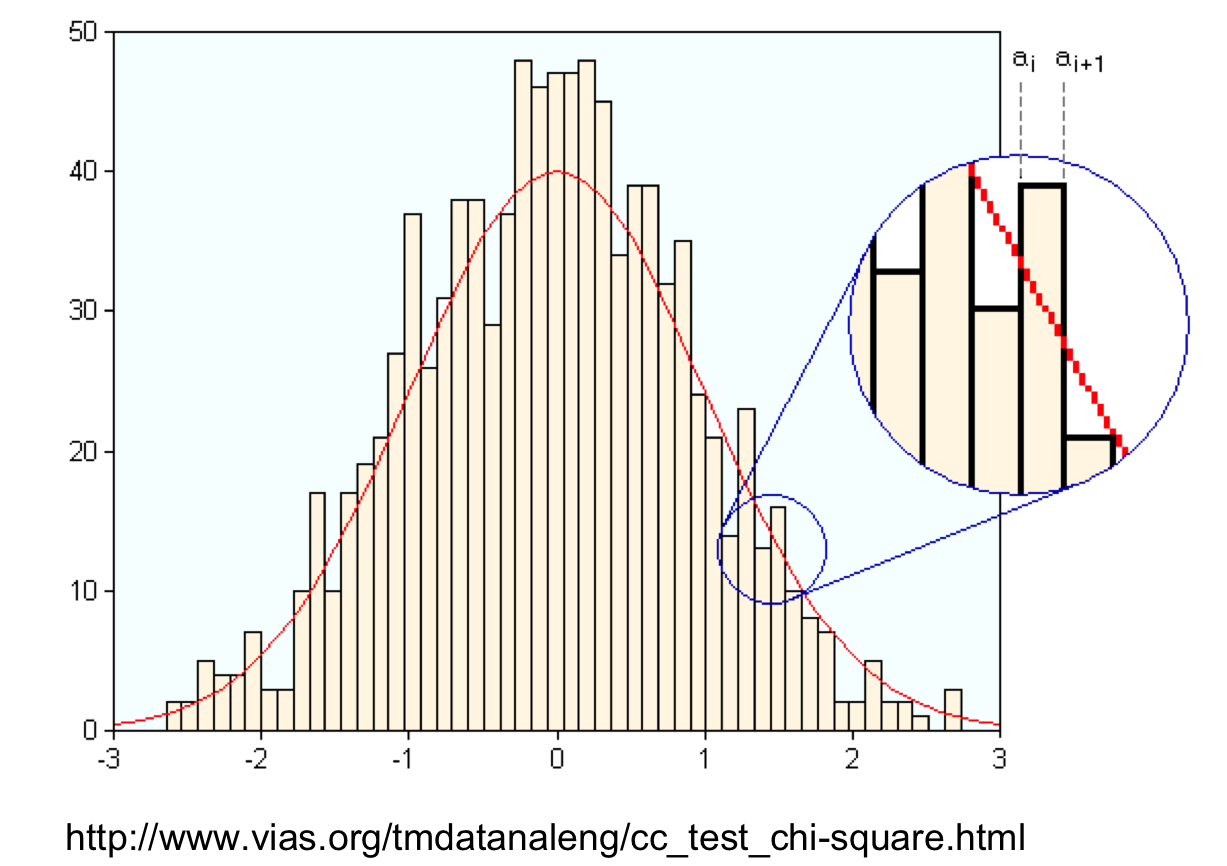
\includegraphics[width=0.8\textwidth]{fig6_chisq.png}
\caption{\label{fig:chisq}Illustration of the $\chi^2$ test of fit between an empirical histogram and a reference pdf.}
\end{figure}

\subsection{Chi-Squared ``Distance''}

$\chi^2$ ``distance'' is a measure of dissimilarity between a pair of histograms.  So there's no theoretical reference and we instead have two empirical histograms.

$$
\chi^2 = \frac{1}{2}\sum_{i=1}^{K} \frac{(F_i - G_i)^2}{F_i+G_i}
$$ where $F_i$, $G_i$ are the two empirical histograms.
Notice that the $\chi^2$ distance doesn't require any sort of ordering at all provided that the word positions in the two histograms correspond with one another. Another note is that $\chi^2$lies between 0 and 1. 

For contrast, consider the $L_2^2$ or Euclidean distance between $F$ and $G$:
$$
L_2^2 = \sum_{i=1}^{K} (F_i - G_i)^2
$$
This looks like the expression for the $\chi^2$ distance without the per-bin normalization term.  As described above for the $\chi^2$ test, the presence of the normalization term emphasizes differences with larger relative significance.  Specifically, two bin counts that are quite large with a difference of $\Delta$ and two bins counts are are rather small with a difference of $\Delta$ are counted in the same manner in the $L_2$ case, whereas the latter gets more weight in the $\chi^2$ case. 

A final note before we move on.  Histograms are nonparametric density estimates.  A normal density, for example, is parametric, with two parameters.  Once you know those, you can specify the entire density.  With a histogram, you instead pick a bin size and count what falls into each bins.  Kernel density estimates are also nonparametric; we can think of it as a smooth counterpart to a histogram, where instead of picking a bin size, we pick a kernel width.  Bernoulli and Multinoulli are parametric.

As a bit of foreshadowing, consider the \emph{Gaussian mixture model}
$$
f(x) = \sum_{m=1}^{M} \alpha_m \phi(x; \mu_m, \Sigma_m)
$$
with $\alpha_m$ representing the mixing proportion $(\sum_m \alpha_m = 1)$, mean $\mu_m$ and covariance $\Sigma_m$.  This is a \emph{semi-parametric} density, a compromise between (nonparametric) KDE, in which every data-point gets a kernel, and (parametric), where one invokes a single density in a one-size-fits-all manner.  We'll see how to fit GMMs in the next lecture.

\section{Cluster Analysis}

Cluster analysis is an unsupervised approach.  The aim of clustering is to partition data into groups such that points in the same group are similar to one another and points in different groups are dissimilar from one another.

There is no ``correct'' clustering.  Nonetheless some solutions are better than others.  It all depends on the measure of dissimilarity.  ``It's the affinities, stupid,'' that is, defining how two points like each other makes the difference--the affinity function.  

An important distinction for clustering is central ($N \times k$ data structure to maintain distances between data points to clusters, as in $k$-means and $k$-medoids) vs.\ pairwise ($N \times N$ data structure to maintain distances between all pairs, as in spectral clustering or graph theoretic).  

%In Figure \ref{fig:kmeans}, you have a scatter that you want to discover groups for that you don't have labels for.  

With central methods, like k-means, you have $N$ data points and $k\ll N$ that are some points of reference or prototypes.  You want to associate all data points with these prototypes to break data into $k$ groups.  The problem is to figure out where the prototype should be and what data points should belong to each group.

It's kind of easy to see how you might cluster two clumps of normally distributed data points using something like $K$-means.  What do you do if one of the groups is instead an annulus, as in Fig.\ \ref{fig:clump_annulus}?  A human observer will recognize two groups, but central clustering methods won't see this since neither group possesses central, prototype points.  Instead, the group membership is propagated from neighbor to neighbor, which we can capture using graph theoretic or pairwise clustering approaches.


\begin{figure}
\centering
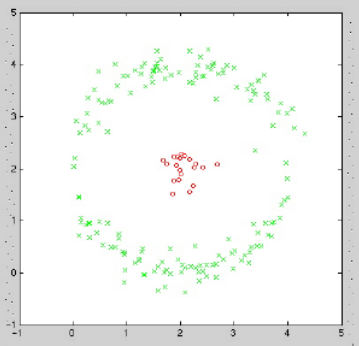
\includegraphics[width=0.4\textwidth]{clump_annulus.png}
\caption{\label{fig:clump_annulus}Example of datapoints arranged in two groups (a clump and an annulus) that aren't well suited to $K$-means clustering.}
\end{figure}


\begin{figure}
\centering
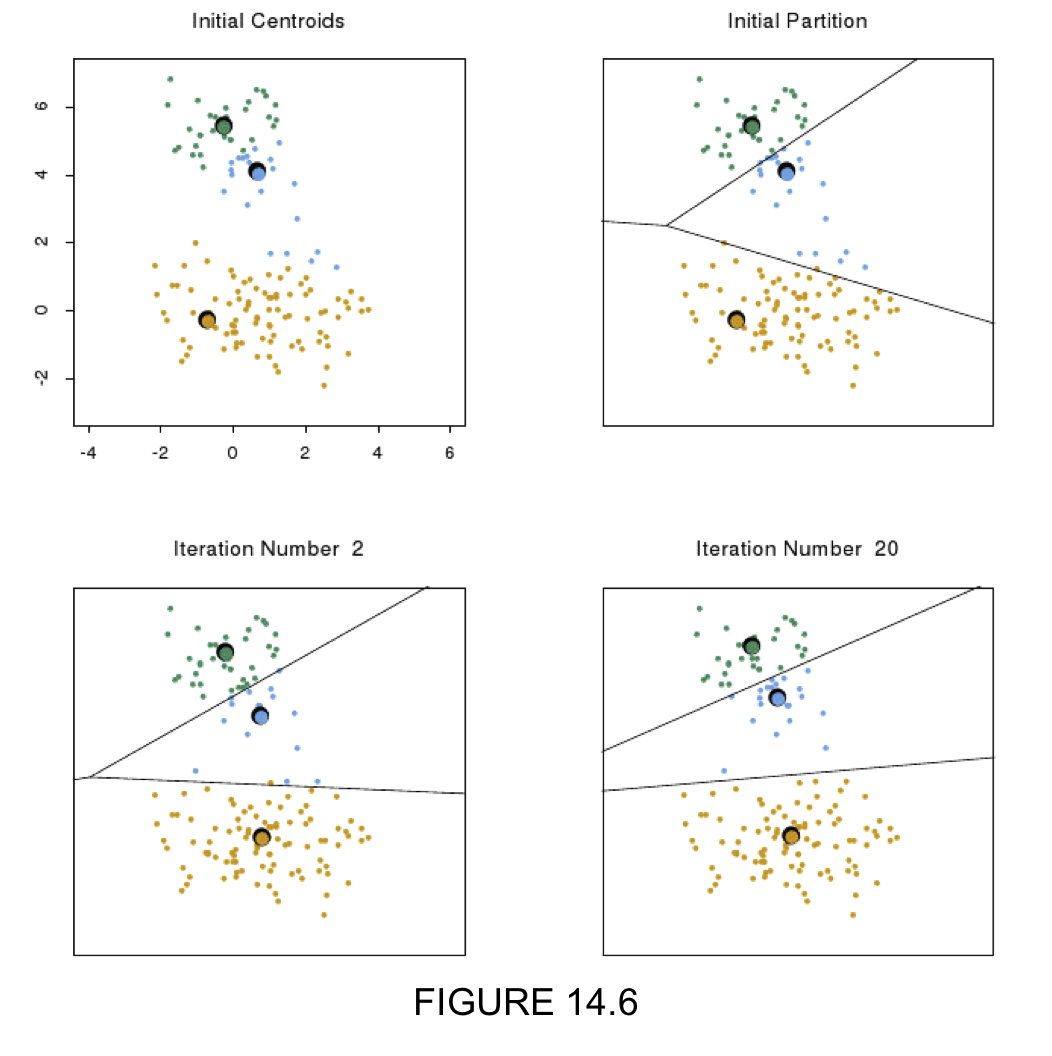
\includegraphics[width=0.8\textwidth]{fig14_6.png}
\caption{\label{fig:kmeans}$K$-means clustering}
\end{figure}



\end{document}
